\documentclass[a4paper, 12pt]{report}

\usepackage[left = 3cm, top = 2.5cm, bottom = 2cm, right = 2cm]{geometry}

\usepackage{graphicx}
\usepackage[spanish,es-tabla]{babel} % Idioma español con tablas

\usepackage{amsmath}
\usepackage{amssymb}
\usepackage{amsfonts}
\usepackage[utf8]{inputenc}         % Para escribir en castellano
\usepackage[T1]{fontenc}
\usepackage{color}
\usepackage{alltt}
\usepackage{times}
\usepackage{latexsym}
\usepackage{anyfontsize}
\setcounter{secnumdepth}{3} %para que ponga 1.1.1.1 en subsubsecciones
\setcounter{tocdepth}{3}    % para que ponga subsubsecciones en el indice
\usepackage{setspace}       % Usado para %\onehalfspace  \doublespacing  \singlespace
\usepackage{booktabs}       % Para formar tablas
%\usepackage{longtable}     % Usado para diseñar grandes tablas.

%\usepackage{algorithmic}
%\usepackage{algorithm}

\usepackage[x11names,table]{xcolor}


%%%%%%%%%%%%%%%%%%%%%%%%%%%%%%%
%%% Tables-related packages %%%
%%%%%%%%%%%%%%%%%%%%%%%%%%%%%%%
%\usepackage{multirow}
%\usepackage{multicol}
%\usepackage{array,colortbl}

\usepackage[round]{natbib} 
\bibliographystyle{apalike}

\usepackage{hyperref}
 
%\newcommand{\yy}{{\'{\i} }}
%\newcommand{\y}{\'{\i}}
%\textheight 21cm

\begin{document}

\baselineskip 1cm
\pagestyle{plain}
%%%%%%%%%%%%%%%%%%%%%%%%%%%%% CARATULA%%%%%%%%%%%%%%%%%%%%%%%%
\textheight 19cm
\pagestyle{empty}
\begin{center}
 {\bf {\fontsize{14}{16.8}\selectfont UNIVERSIDAD NACIONAL DE TRUJILLO}}     
 
    {\bf{\fontsize{14}{16.8}\selectfont Facultad de Ciencias Físicas y Matemáticas}} 

  {\bf{\fontsize{14}{16.8}\selectfont Escuela Profesional de Informática}}
\end{center}  

\begin{figure}[ht]
\begin{center}

\includegraphics[width=.4\textwidth]{unt}
\end{center}
\end{figure}

\vskip 2cm
\begin{center}
  { \bf {\fontsize{17}{20.4}\selectfont{MODELO PARA LA RUTERIZACIÓN }}     
  \vskip 3cm
  {\bf \fontsize{14}{16.8}\selectfont {Edgar Peche Perlado}}} \\
    %{\bf \fontsize{14}{16.8}\selectfont {Manuel Perez Yon}} 

\end{center}   
\vskip 1.3cm
\begin{center}    
{\bf {\fontsize{14}{16.8}\selectfont Trujillo - La Libertad
\vskip 0.0cm
\hspace*{-0.2cm} 
2018 }}
\end{center} 
\newpage
%%%%%%%%%%%%%%%%%%%%%%%%%%%%%%%%%%%%%%%%%%%%%%%%%%%%%%%%%%%%%%%%%%%%%%%%%%%


%%%%%%%%%%%%%%%%%%%%%%%%%%%%CONTRA CARATULA 1 %%%%%%%%%%%%%%%%%%%%%%%%%%%%%
\newpage
\pagestyle{plain}
\pagenumbering{roman}

\hspace*{6cm}
\vskip 9cm
\begin{center}
   {\bf \doublespacing {\fontsize{17}{20.4}\selectfont{MODELO PARA LA RUTERIZACIÓN }}}     
\end{center} 
\newpage
%%%%%%%%%%%%%%%%%%%%%%%%%%%%%%%%%%%%%%%%%%%%%%%%%%%%%%%%%%%%%%%%%%%%%%%%%%%


%%%%%%%%%%%%%%%%%%%%%%%%%%%%% CONTRA CARATULA 2 %%%%%%%%%%%%%%%%%%%%%%%
\begin{center}
   {\bf {\fontsize{14}{16.8}\selectfont{EDGAR PECHE PERLADO}}}\\    
      %{\bf {\fontsize{14}{16.8}\selectfont{MANUEL PEREZ YON}}}       
   \end{center}   

\vskip 3.2cm
\begin{center}
   {\bf \doublespacing {\fontsize{17}{20.4}\selectfont{MODELO PARA LA RUTERIZACIÓN }}}     
\end{center}   
  \vskip 2cm
\begin{verse}
 \fontsize{12}{14.4}\selectfont{\hspace*{0.6cm}Informe de suficiencia profesional presentada a la Escuela Profesional de Informática en la Facultad de Ciencias Físicas y Matemáticas de la Universidad Nacional de Trujillo, como requisito parcial para la obtención del Título profesional de Ing. Informático}
\end{verse}

\vskip 1.5cm 
{\fontsize{14}{16.8}\selectfont ASESOR: JOSÉ A. RODRIGUEZ MELQUIADES} 
 \vskip 1cm 
 \begin{center}    
 \vskip 2cm
{\fontsize{14}{16.8}\selectfont Trujillo - La Libertad
\vskip 0.2cm
\hspace*{-0.2cm} 
2018}
\end{center} 
\newpage
%%%%%%%%%%%%%%%%%%%%%%%%%%%%%%%%%%%%%%%%%%%%%%%%%%%%%%%%%%%%%%%%%%%%%%%%%%%%%


%%%%%%%%%%%%%%%%%%%%%%%%%%%%HOJA DE APROBACION %%%%%%%%%%%%%%%%%%%%%%%%%%%%%
\begin{center}
 {\bf {\Large HOJA DE APROBACIÓN }     
 \vskip 1.5cm
  {\Large Modelo para la Ruterización }}
 \vskip 1cm 
  {\large{Edgar Peche Perlado}}\\
    %{\large{Manuel Perez Yon}}

 \vskip 1cm
\end{center} 
Informe de suficiencia profesional defendida y aprobada por el jurado examinador:
\vskip 1.5 cm
\begin{flushleft} 
$\overline{\mbox{Prof. Dr. José A. Rodríguez Melquiades}}$\\
\vskip -0.5cm
Departamento de Informática - UNT
\end{flushleft} 
\vskip 1cm
\begin{flushleft} 
$\overline{\mbox{Prof. Mg. Christian Araujo Gonzales}}$\\
\vskip -0.5cm
Departamento de Informática - UNT
\end{flushleft} 
\vskip 1cm
\begin{flushleft} 
$\overline{\mbox{Prof. Mg. Juán O. Salazar Campos}}$\\
\vskip -0.5cm
Departamento de Informática - UNT
\end{flushleft}
\vskip 0.8cm 
\begin{center}    
Trujillo, 23 de diciembre del 2018
\end{center} 
\newpage
%%%%%%%%%%%%%%%%%%%%%%%%%%%%%%%%%%%%%%%%%%%%%%%%%%%%%%%%%%%%%%%%%%%%%%%%%%%%


%%%%%%%%%%%%%%%%%%%%%%%%%%%% DEDICATORIA %%%%%%%%%%%%%%%%%%%%%%
 
 \addcontentsline{toc}{chapter}{Dedicatoria}
 {\bf\Large {Dedico este informe de suficiencia profesional a :}}
 \vskip 1cm
\begin{quotation}
{\it Mis padres ....
\vskip 1cm
Mi hemano ... .
\vskip 1cm
Mi ... .}
\end{quotation}
%%%%%%%%%%%%%%%%%%%%%%%%%%%%%%%%%%%%%%%%%%%%%%%%%%%%%%%%%%%%%%%%%%%%%%%%%%%


%%%%%%%%%%%%%%%%%%%%%%%%%%%% AGRADECIMENTOS %%%%%%%%%%%%%%%%%%%%%%
\newpage

 \addcontentsline{toc}{chapter}{Agradecimientos}
 {\bf\Large {\flushleft{Agradecimientos}}}
 \vskip 1.5cm
\begin{quotation}
Agradezco a Dios por haberme bendecido en toda mi vida ....
{\vskip 1cm}
A mis profesores del Departamento de Informática, de los cuales recibi una gran cantidad de conocimientos  . . .
\vskip 1cm
%A mi asesor Prof. Dr. José A. Rodríguez Melquiades que siempre se mostro disponible e interesado en ayudarme.
\vskip 1cm
 . . .
 \end{quotation}
%%%%%%%%%%%%%%%%%%%%%%%%%%%%%%%%%%%%%%%%%%%%%%%%%%%%%%%%%%%%%%%%%%%%%%%%%%%


%%%%%%%%%%%%%%%%%%%%%%%%%%%% RESUMEN%%%%%%%%%%%%%%%%%%%%%%
\newpage
\begin{center}
 \addcontentsline{toc}{chapter}{Resumen}
 {\bf\LARGE Resumen}
\end{center} 
\vskip 0.5cm
\begin{quotation}
{\bf Ejemplo:}\par

La investigación bibliográfica revela una preocupación de los gobiernos federales en lo relacionado al destino final de los residuos sólidos urbanos (RSU), con el objetivo de preservar la salud de la población, el medio ambiente urbano y rural. En este contexto y para el caso de las ciudades brasileras se esperaba que con la desactivación legal de los botaderos hasta el año 2014, surgiesen medidas que viabilicen la colecta selectiva, reciclaje y reutilización para aproximadamente el $80\%$ del volumen total de residuos colectados y destinados a locales no apropiados. 
\vskip 0.2cm 
En este sentido esta investigación tiene como objetivo principal modelar y planificar una red de logística reversa para una región urbana, dimensionando el flujo de RSU que será movido a lo largo de la red, el número y capacidad de las estaciones de colecta, de las unidades productivas y especiales necesarias para su colecta, transporte y disposición final. Los resultados muestran que es posible realizar un modelo matemático para este tipo de problemas, así como su aplicación en diversas regiones sin necesidad de grandes cambios en el modelo propuesto.    

\vskip 0.3cm
\hspace*{-0.6cm}{\bf Palabras claves:} residuos sólidos urbanos, logística reversa, modelo matemático.
\end{quotation}
%%%%%%%%%%%%%%%%%%%%%%%%%%%%%%%%%%%%%%%%%%%%%%%%%%%%%%%%%%%%%%%%%%%%%%%%%%%%%%%%%%%%


%%%%%%%%%%%%%%%%%%%%%%%%%%%%ABSTRACT%%%%%%%%%%%%%%%%%%%%%%
\newpage
\begin{center}
 \addcontentsline{toc}{chapter}{Abstract}
 {\bf\LARGE Abstract}\vskip 1.5cm
\end{center} 
\begin{quotation}

{\bf Ejemplo:}\par

The literature reveals a concern of Federal Governments with the disposal of municipal solid waste (MSW) in order to preserve the health of the population, the urban and rural environment. In this context and for the case of Brazilian cities, it was expected that, with the legal command for the deactivation of landfills by 2014, measures would be adopted in order to enable the selective collection, recycling and reuse for about $80\%$ of the total volume of collected solid waste and intended to inappropriate places. 
\vskip 0.2cm
In this sense, this research aims to model and plan a reverse logistics network to an urban area, dimensioning the flow of MSW that will be moved along the network, the number and capacity of collection stations, and the productive and special units required for their collection, transportation and final disposal. The results show to be possible perform mathematical modeling of this problem with low investment, as well as apply it in various regions without major changes in the proposed model.

\vskip 0.3cm
\hspace*{-0.6cm}{\bf Keywords:} solid waste, reverse logistics, mathematical modeling.
\end{quotation}
%%%%%%%%%%%%%%%%%%%%%%%%%%%%%%%%%%%%%%%%%%%%%%%%%%%%%%%%%%%%%%%%%%%%%%%%%%%%%%


%%%%%%%%%%%%%%%%%%%%%%%%%%% LISTA DE SIMBOLOS %%%%%%%%%%%%%%%%%%%%%%
\newpage
\addcontentsline{toc}{chapter}{Lista de símbolos}
 {\bf\LARGE Lista de símbolos}
 \vskip 1.5cm
Constantes: 
\begin{enumerate}
\item[(1)]$r,\overline{r} $ \hspace*{0.8cm} Indice que denota regiones.
\item[(2)] $n $ \hspace*{1.1cm} Indice de bienes finales deseados por los consumidores.
\item[(3)] ...
\vskip 3cm
\end{enumerate} 
\vskip 0.3cm
Variables:
\begin{enumerate}
\item[(5)] $ x^{r} $ \hspace*{1cm} Vector columna que denota la actividad de producción.
\item[(6)] $ u^{r} $ \hspace*{1.2cm} . . .
\end{enumerate}
            % Datos de la tesis
\listoffigures               % indice de figuras
\addcontentsline{toc}{chapter}{Índice de Figuras}
\listoftables                % indice de tablas
\addcontentsline{toc}{chapter}{Índice de Tablas}
\tableofcontents             % indice de materias
\chapter{Record laboral}
\pagenumbering{arabic}
\setcounter{page}{1}
%\renewcommand{\baselinestretch}{2} %doble espacio paratodo el texto

%Describir su participación en la empresa donde laboro, indicar uno o dos empresas, indicando la siguiente información:   

\section{Imagina Technologies}


\subsection{Cargo desempeñado}
Programador Web

\subsection{Descripción del cargo desempeñado}
Desarrollo de aplicaciones Web usando HTML, Javascript y PHP. Además, creación de procedimientos almacenados en MySQL.

\subsection{Lugar y fecha}
El vínculo laboral se desarrolló en la ciudad de Trujillo (Perú) desde Mayo hasta Octubre del 2015.

\section{Everis}

\subsection{Cargo desempeñado}
Programador SAP/ABAP y Líder de equipo

\subsection{Descripción del cargo desempeñado}
Desarrollo de aplicaciones SAP, especialmente en los módulos FI(Finanzas) y MM (Materiales). Además, responsable por la gestión de equipos y capacitación de los nuevos miembros.

\subsection{Lugar y fecha}
El vínculo laboral se desarrolló en la ciudad de Trujillo (Perú) desde Mayo del 2017 hasta Agosto del 2019.

\section{Level33}

\subsection{Cargo desempeñado}
Programador Full Stack y Líder de equipo

\subsection{Descripción del cargo desempeñado}
Desarrollo de aplicaciones Web y Mobile para órganos del gobierno, Así como, coordinación de equipos con miembros de diferentes nacionalidades y solución de dudas técnicas.

\subsection{Lugar y fecha}
El vínculo laboral se desarrolló en la ciudad de Brasilia (Brasil) desde Agosto del 2019 hasta Agosto del 2020.

\section{BrScan}

\subsection{Cargo desempeñado}
Desarrollador Web

\subsection{Descripción del cargo desempeñado}
Desarrollo, manutención y mejora de aplicativos web usando Angular y PHP. Asimismo, aplicación de procesos ágiles en el desenvolvimiento.

\subsection{Lugar y fecha}
El vínculo laboral se desarrolla en la ciudad de Brasilia (Brasil) desde Septiembre del 2020 hasta la actualidad.


\chapter{Memoria descriptiva}

%Debe detallar todas las tareas y trabajos ejecutados como parte de las labores realizadas en cada uno de los centros laborales acreditados.\par
%\vskip 0.1cm
%Esta relación se presentará de manera ordenada y sistemática, siguiendo un orden cronológico. Se debe acreditar con constancias emitidas de cada una de las instituciones de las que se presentan constancias de trabajo. Seguir el formato siguiente.

\section{Imagina Technologies}

\subsection{Descripción de la empresa}
%Descripción (razón social, RUC, dirección, rubro, organigrama) 

IMAGINA TECHNOLOGIES S.A.C. con RUC 20600064941 ubicada en Av. Húsares de Junin 1203 Ofic. 401 Trujillo - Perú; empresa dedicada al desarrollo de software para grandes, medianas y pequeñas empresas, trabajando bajo metodologías, estándares de calidad y prácticas de empresas de servicios de TI. Imagina Technologies ofrece soluciones de TI adaptadas al negocio del cliente. El objetivo de la empresa es aumentar los diferenciadores de mercado del cliente, hacerlo más productivo y competitivo. 

\subsection{Web de la empresa}
\url{http://itecsac.com/}

\subsection{Nombre del área}
%Descripción (funciones del área-organigrama) 
Gerente -> Fabrica de software -> Jefe de Proyecto -> Programadores


\subsection{Nombre del cargo}
Programador Web

\subsubsection{Descripción del cargo ocupado dentro de la empresa} 
Desarrollo de aplicaciones Web usando HTML, Javascript y PHP. Además, creación de procedimientos almacenados en MySQL.

\subsubsection{Actividades desarrolladas en la empresa} 
\begin{itemize} 
	
\item Desarrollo y mantenimiento de sistemas web para empresas de la ciudad utilizando PHP, XML, Javascript, JSON, Ajax y JQuery.
\item Creación de procedimientos almacenados en MYSQL.
\item Optimización del "homemade' framework basado en PHP.
\item Creación de interfaces web responsivas usando Bootstrap.
%- Instalación de los sistemas para los usuarios.
\end{itemize} 


\subsubsection{Logros obtenidos dentro de la empresa} 

\begin{itemize} 
\item blablabla
\item blablabla
\item blablabla	
\end{itemize} 

\subsubsection{Resultados obtenidos dentro de la empresa} 

\begin{itemize} 
	\item blablabla
	\item blablabla
	\item blablabla	
\end{itemize} 

\subsection{Datos del jefe inmediato superior}

\subsubsection{Nombres y apellidos}
Heredia Lozada Christopher Segundo 

\subsubsection{Cargo} 
Gerente / Jefe de Proyecto 

\subsubsection{Correo electrónico} 
HerediaLozadaChristopherSegundo@imaginatecperu.com 
comercial@imaginatecperu.com 

\subsubsection{Teléfono} 
+51 94205-1234


%%%%%%%%%%%%%%%%%%%%%%%%%%%%%%%%%%%%%%%


\section{Everis}

\subsection{Descripción de la empresa}
Everis Peru S.A.C. con RUC 20521586134 ubicada en Calle Dean Valdivia 148 Torre 1 Piso 4 URB. Los Jardines, San Isidro, Lima - Perú; empresa dedicada a la consultoría y outsourcing abarcando todos los sectores del ámbito económico, llegando a facturar en el último ejercicio fiscal 1.454 millones de euros, formada por más de 27.000 profesionales repartidos por Europa, USA y Latinoamérica.

\subsection{Web de la empresa}
\url{https://www.everis.com/peru/es/home-peru}

\subsection{Nombre del área}
%Descripción (funciones del área-organigrama) 
TTL -> CSD -> CD -> CJ

\subsection{Nombre del cargo}
Center Senior Developer

\subsubsection{Descripción del cargo ocupado dentro de la empresa} 
Desarrollo de aplicaciones SAP, especialmente en los módulos FI (Finanzas) y MM (Materiales). Además, responsable por la gestión de equipos y capacitación de los nuevos miembros.

\subsubsection{Actividades desarrolladas en la empresa}

\begin{itemize} 
	\item Participación en la implementación de software SAP en los módulos FI y MM.
	\item Responsable por la coordinación de equipos en los proyectos.
	\item Capacitación y dictado de aulas sobre el lenguaje de programación ABAP.
	\item Integración continua con tecnología SAP WEB: HTML5 y Javascript.
\end{itemize} 


\subsubsection{Logros obtenidos dentro de la empresa} 

\begin{itemize} 
	\item Promoción de categoría CJ(Center Junior) a moo(Center Developer) en un tiempo menor al plazo estipulado debido al buen desempeño.
	\item Asignación como instructor para el programa de capacitación a los nuevos postulantes.
	\item Reconocimiento por parte de gerencia debido a la presentación del proyecto "Working Capital" para la sucursal de Argentina.	
\end{itemize} 

\subsubsection{Resultados obtenidos dentro de la empresa} 
\begin{itemize} 
	\item Entrega de proyectos antes del plazo final.
	\item Incremento del desempeño de los nuevos trabajadores debido a la capacitación impartida.
	\item Notable presentación del proyecto "Working Capital" para los stakeholder.	
\end{itemize} 

\subsection{Datos del jefe inmediato superior}


\subsubsection{Nombres y apellidos} 
Edgar Cubas Rubio 

\subsubsection{Cargo}
Technical Team Leader

\subsubsection{Correo electrónico} 
Edgar.cubas.rubio@everis.com

\subsubsection{Teléfono} 
+51 94932-2432

%%%%%%%%%%%%%%%%%%%%%%%%%%%%%%%%%%%%%%%


\section{Level33}

\subsection{Descripción de la empresa}
Level 33 comércio e serviço de tecnologia LTDA con CPNJ 09.078.124/0001-64 ubicada en SIG conjunto D lote 11 Brasília - DF, Brasil; esta empresa es una startup dedicada al desarrollo de aplicativos web y móviles, teniendo como principales clientes entidades gubernamentales en los diferentes estados de Brasil. 

\subsection{Web de la empresa}
\url{www.level33.com.br}

\subsection{Nombre del área}
%Descripción (funciones del área-organigrama) 
Gerente -> Jefe de Projecto -> Testers y Programadores


\subsection{Nombre del cargo}
Desenvolvedor Full Stack

\subsubsection{Descripción del cargo ocupado dentro de la empresa}
Desarrollo de aplicaciones Web y Mobile para órganos del gobierno, Así como, coordinación de equipos con miembros de diferentes nacionalidades y solución de dudas técnicas.

\subsubsection{Actividades desarrolladas en la empresa} 

\begin{itemize} 
	\item Creación y manutención de aplicaciones web y móviles para órganos del gobierno y sector privado.
	\item Gestión del equipo de desarrolladores de diferentes nacionalidades.
	\item Análisis y diseño de soluciones técnicas, ademas implantación de mejores practicas.
	\item Solución de dudas técnicas.
\end{itemize} 

\subsubsection{Logros obtenidos dentro de la empresa} 

\begin{itemize} 
	\item Implementación de la metodología SCRUM en la empresa.
	\item Asignación como líder y instructor del equipo de programadores. 
	\item Extender el uso de un sistema controlador de versiones por todo el equipo.
\end{itemize} 

\subsubsection{Resultados obtenidos dentro de la empresa}

\begin{itemize} 
	\item Entrega de los proyectos en los plazos indicados.
	\item Disminución de bugs en las aplicaciones desarrolladas por el equipo de programadores.
	\item Organizado y rápido acceso al código fuente de los proyectos.
\end{itemize} 

\subsection{Datos del jefe inmediato superior}

\subsubsection{Nombres y apellidos} 
Paulo Fernandes

\subsubsection{Cargo}
Jefe de proyecto.

\subsubsection{Correo electrónico} 
pfernandes@tecnew.com.br

\subsubsection{Teléfono} 
+55 61 99221-8407

%%%%%%%%%%%%%%%%%%%%%%%%%%%%%%%%%%%%%%%

\section{BrScan}

\subsection{Descripción de la empresa}
BrScan processamento de dados e tecnologia LTDA con CPNJ 06.198.573/0001-58 ubicada en SETOR SCS QUADRA 02 BLOCO C Brasília - DF, Brasil; empresa dedica da a la creación de aplicaciones de gestión desde el 2004 enfocada a trabajar con soluciones de gestión de riesgo documental, de información y seguridad en los procesos organizacionales. 


\subsection{Web de la empresa}
\url{https://www.brscan.com.br/}

\subsection{Nombre del área}
%Descripción (funciones del área-organigrama) 
driJefe de Projecto -> Testers y Programadores


\subsection{Nombre del cargo}
Desarrollador Web

\subsubsection{Descripción del cargo ocupado dentro de la empresa}
Desarrollo, manutención y mejora de aplicativos web usando Angular y PHP. Asimismo, aplicación de procesos ágiles en el desenvolvimiento.

\subsubsection{Actividades desarrolladas en la empresa} 
\begin{itemize} 
	\item Creación y manutención de módulos en los aplicativos de la empresa.
	\item Aplicación de procesos ágiles como SCRUM.
	\item Soporte al equipo de base de datos.
\end{itemize} 

\subsubsection{Logros obtenidos dentro de la empresa}
\begin{itemize} 
	\item Aprendizaje del flujo de negocio de los aplicativos en corto tiempo.
	\item blablabla
	\item blablabla
\end{itemize}  

\subsubsection{Resultados obtenidos dentro de la empresa} 
\begin{itemize} 
	\item Entrega de las asignaciones en el tiempo indicado.
	\item blablabla
	\item blablabla
\end{itemize} 


\subsection{Datos del jefe inmediato superior}

\subsubsection{Nombres y apellidos} 
Mauro Rodrigues Nogueira

\subsubsection{Cargo} 
Líder de proyecto

\subsubsection{Correo electrónico} 
mauro.rodrigues@brscan.com

\subsubsection{Teléfono} 
+55 61 99238-5259


%%%%%%%%%%%%%%%%%%%%%%
%%%%%%%%%%%%%%%%%%%%%%
%%%%%%%%%%%%%%%%%%%%%%



\chapter{Experiencia profesional}
De las labores referidas en la memoria descriptiva, el bachiller elegirá una de ellas la que al ser ampliada y detallada se presentará para la sustentación correspondiente. Este informe deberá contemplar los siguientes aspectos:

\section{Fundamentación}

\subsection{Realidad problemática}
%Conocimiento de la realidad donde la empresa hizo un estudio e identifico una problemática, para un posterior aporte informático.
Una de las ciudades mas ricas de Brasil, Brasilia, esta desenvolviendo um ecosistema de Start-ups, el cual a pesar de ser joven lidera el mercado de centro oeste brasileño gracias a la creciente economía de la ciudad. Sin embargo, la rápida evolución tiene sus inconvenientes siendo el mas común la falta de organización en sus procesos internos todas sobre todo en la Start-ups que ubicadas en los alrededores de Brasilia en las llamadas "ciudades satélite. La Start-up de TI en la cual realice mi intercambio laboral se ubicada en unas de estas ciudades, usa como principal mano de obra intercambistas extranjeros y no contaba con ninguna metodología para regular sus procesos a la hora de realizar un proyecto y lograr las entregas en el tiempo estipulado.


\subsection{Formulación del problema}
{\bf Ejemplo:}\par

  En este trabajo, se propone la implementación de la metodología SCRUM  en una startup brasileña para responder a la siguiente pregunta:
 \begin{center} 
     ?`Cómo organizar una estructura/plan para concluir proyectos en los plazos establecidos siguiendo una metodología ágil ?
 \end{center}


\subsection{Justificación practica}

Este trabajo se realiza porque existe la necesidad de implementar una metodología ágil para organizar los procesos en una startup y de ese modo poder tener un flujo claro de la planificación y el cumplimiento de los plazos de entrega de los proyectos.


\subsection{Limitaciones}
En la realización de este trabajo encontramos algunas limitaciones, por ejemplo:

\begin{itemize} 
	\item La falta de personal con habilidades de capacitación en la startup.
\end{itemize} 


\subsection{Objetivos}
Es necesario establecer
 qué pretende la investigación, es decir, cuáles son sus objetivos. Hay investigaciones que buscan contribuir a resolver un problema en especial, y otras tienen como objetivo principal probar una teoría o aportar evidencia empírica en favor de ella. \par 
\vskip 0.3cm
Segun \cite{Rojas}, los objetivos tienen que expresarse con claridad para evitar posibles desviaciones en el proceso de investigación y deben ser susceptibles de alcanzarse; son las guías del estudio y hay que tenerlos presentes durante todo su desarrollo. Los objetivos deben ser congruentes entre sí.
\vskip 0.3cm
Describir el objetivo central o propósito del proyecto de investigación (debe estar alineado con el problema e hipótesis), así como los objetivos específicos, los cuales deben reflejar los cambios que se esperan lograr en trabajo de tesis (variables). Para estos objetivos específicos utilice verbos como: describir, indicar, modificar, controlar, producir (tecnologías), recuperar, etc..

\subsubsection{Generales}
Debe explicitar lo que se espera lograr con el estudio en términos de conocimiento. Debe dar una noción clara de lo que se pretende describir, determinar, identificar, comparar y verificar.


\subsubsection{Específicos}
Son la descomposición y secuencia lógica del objetivo general. Son un anticipo del diseño de la investigación.
\vskip 0.3cm


{\bf Ejemplo de objetivos:}\\
{\bf Objetivo General:}
\begin{enumerate}
\item[a)] La investigación tiene como objetivo principal modelar y planificar una red logística reversa para una región urbana, dimensionando el flujo de RSU que será transportado a lo largo de la red y determinar el número y capacidad de las estaciones de colecta y de la unidades productivas y especiales necesarias para la atención de la región, en cuanto a la colecta, transporte y disposición final de los RSU.
\vskip 0.3cm
\item[b)]Con la optimización del modelo de colecta de RSU, es posible reorganizar el sistema logístico reverso de una ciudad de forma que se consiga un mejor dimensionamiento de la red, con la consecuente disminución del número que circulan en la ciudad.
\end{enumerate}
\vskip 0.2cm
{\bf Objetivos específicos:}
\begin{enumerate}
\item[a)] Aplicar una metodología de programación lineal entera, considerada computacionalmente como un problema que pertenece a la clase de complejidad NP \citep{Korte} para solucionar el problema.
\item[b)] Implementar con CPLEX, rodando en el sistema operativo Linux, los modelos propuestos, validarlos y testarlos en un caso práctico.
\end{enumerate}


\subsection{Planteamiento de la solución}
Debe indicar como va a resolver la problematica planteada, es decir, con que base teórica y herramientas computacionales resolvera los problemas en la empresa donde labora o laboró.


\subsection{Análisis de Viabilidad (Operativa, económica, tecnológica, social, etc.)}

\subsection{Recursos (Humanos, Hardware, Software, Materiales, Servicios)}

\subsection{Presupuesto}

\subsection{Cronograma}


\section{Desarrollo de la solución}
Desarrollo de la problemática planteada mediante el uso alguna metodología y/o conocimiento científico usado para el bienestar de la sociedad.


\subsection{Problemas combinatorios}
\subsection{Heurísticas y metaheurísticas}

\subsection{Sustentabilidad}

{\bf Ejemplo:}\par

La configuración, característica, jurisdicción administrativa, relaciones económicas, sociales y ambientales de un espacio urbano se define por la población y por la función que ella desarrolla en un área geográfica o región \citep{Bugliarello}. De este modo las ciudades son sistemas dinámicos que interactúan continua y constantemente con su medio ambiente, acompañando las características, perfil, cultura y ritmo de desarrollo económico y social de su población. Los medios de transporte juegan un papel importante en tal ritmo de desarrollo de las ciudades, ya que ellos tienen como función relacional los factores poblacionales con los factores uso del suelo.  
\vskip 1cm
El desarrollo sustentable, (Figura 2.1), estará garantizado si se consideran tres aspectos fundamentales: económico, social y ambiental, donde la intersección de estos aspectos garantiza la calidad de vida en el espacio urbano y el equilibrio en las clases sociales en busca del bienestar \citep{Tanguay}.

\begin{figure}[ht]
\begin{center}
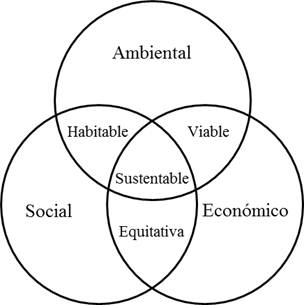
\includegraphics[width=0.3\textwidth]{Figura2}
\end{center}
\begin{center}
\vskip -0.5cm
\caption{\small{Aspectos claves para el desarrollo sustentable.}}
{\small{Fuente: \cite{Tanguay}}}
\end{center}
\end{figure}

\subsection{Logística directa y reversa}

\subsubsection{Logística directa}

{\bf Ejemplo:}\par

\cite{Ghiani} entienden que la logística trata de la planificación y control de los flujos de materiales e informaciones relacionadas en las organizaciones, tanto en los sectores público y privado. Además su misión es hacer la entrega de los productos correctos, en el local correcto y en la hora correcta, optimizando los costos operacionales totales del proceso.
satisfaciendo un determinado conjunto de restricciones o condiciones.\par

\subsubsection{Logística reversa}

{\bf Ejemplo:}\par

En los años 90 se presentaron definiciones generales las cuales vienen siendo mejoradas. \cite{Dekker} presenta una mejora en la definición de logística reversa como  ”el proceso de planificación, implementación y control de los flujos de materias-primas, en procesos de inventarios y bienes acabados, desde el punto de fabricación, distribución o uso, hacia el punto de recuperación o de eliminación”. 
\begin{figure}[ht]
\begin{center}
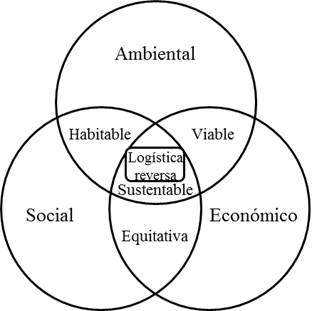
\includegraphics[width=0.3\textwidth]{Figura1}
\end{center}
\begin{center}
\vskip -0.5cm
\caption{\small{Logística reversa incluida en el desarrollo sustentable.}}
{\small{Fuente: Adaptación de \cite{Tanguay}}}
\end{center}
\end{figure}


\subsubsection{Modelos}

\subsection{Modelamiento y ruteo }

{\bf Ejemplo:}\par

El modelamiento matemático es una alternativa para expresar formalmente hechos reales que pueden ayudar en el proceso de toma de decisiones. El modelamiento permite la simulación de procesos  y de escenarios con la introducción de índices de desempeño que permitan cuantificar los costos y beneficios de la implementación del sistema, la mejoría de la sustentabilidad urbana y por supuesto los índices de contaminación en las grandes ciudades y su impacto en todo el medio ambiente. 

\subsubsection{Modelos utilizados en los problemas de ruteo de vehículo }

{\bf Ejemplo:}\par

El problema de ruteo de vehículos \citep{Ombuki, Yeun} y sus variantes han ganado mucho interés en la comunidad académica. La intención de estar más cerca a la realidad mediante el modelamiento matemático, hace que se hayan desarrollado nuevos modelos de optimización. \par
\vskip 0.3cm
Según \cite{Sterle} el primer nivel de la red comprende la distribución de la carga desde las plataformas hasta las unidades satélites, utilizando vehículos de carga de mayor tamaño (g).  El segundo nivel, consiste en montar rutas desde las unidades satélites hasta los clientes, usando para este caso vehículos de menor tamaño (v). El modelo de localización y ruteo de vehículos para la distribución de carga propuesto por el autor, además de hacer la conexión de los dos niveles y estudiar su inter relación y dependencia, el modelo busca determinar la cantidad necesaria de plataforma y de unidades satélites considerando el tamaño y dimensionamiento de la flota para el ruteo en dos niveles. 
\vskip 0.2cm

\begin{table}[h!]
\begin{center}
\caption{\small{Resultados computacionales obtenidos en el modelo de \cite{Sterle}}}
\end{center}
\vskip -0.7cm
\begin{tabular}{|c|c|c|c|c|}
\hline 
\rowcolor{LightBlue2}{\small Escenarios} & {\small Demanda cliente (ton.)} & {\small Tiempo (min.)} & {\small Costo ($\$$)} \\ 
\hline 
{\small 1} & {\small P1:1; P2:2; P3:2; P4:2; P5:1} & {\small 0.12} & {\small 667.42} \\ 
\hline 
{\small 2} & {\small P1:1; P2:2; P3:2; P4:2; P5:1; P:4; P7:3} & {\small 56.54} & {\small 1744.35} \\ 
\hline 
{\small 3} & {\small P1: 1; P2:2; P3:2; P4:2; P5:1; P6: 4; P7:3; P8:2; P9:2} & {\small 287.70} & {\small 1750.72} \\ 
\hline 
{\small 4} & {\small P1:1; P2:2; P3: 2; P4:2; P5:1; P6:4; P7:3; P8:2; P9:2; P10:1} & {\small 1848.57} & {\small 1773.46} \\ 
\hline 
{\small 5} & {\small P1:1; P2:2; P3: 2; P4:2; P5:1; P6:4; P7:3; P8:2; P9:2; P10:1} & {\small 1848.57} & {\small 1773.46} \\ 
\hline 
{\small 6} & {\small P1:1; P2:2; P3: 2; P4:2; P5:1; P6:4; P7:3; P8:2; P9:2; P10:1} & {\small 1848.57} & {\small 1773.46} \\ 
\hline 
\end{tabular} 
\begin{center}
\vskip -0.2cm
{\small{Fuente: Resultados obtenidos con CPLEX.}}
\end{center}
\end{table}


\chapter{Resultados obtenidos con la experiencia profesional en la empresa}


Al culminar con el desarrollo de la experiencia profesional en la solución de la problemática encontrada en la sociedad, se llegaron a resultados interesantes del punto de vista tanto teórico como computacional. Estos resultados muestran que se contrasta la solución planteada, es decir, que se logró demostrar la relación entre las variables de estudio formuladas en la experiencia.

\section{Teóricos y/o académico}

\section{Resultados computacionales y/o aplicativa y/o valorativo.}




\chapter{Consideraciones finales}

\section{Conclusiones}

{\bf Ejemplo}\\
La investigación bibliográfica revela que realmente existe una preocupación de los gobiernos federales con el destino final de los residuos sólidos, con el objetivo de preservar la salud de la población y el medio ambiente urbano y rural. Por ejemplo, se observa la creación, en el caso del Brasil, de la Ley 12.305/10. Sin embargo existe una laguna entre las metas propuestas en la ley con las metas reales de los gobiernos locales. Eso se debe a la falta de una buena estructura organizacional, gerencial y operacional de los gobiernos locales capaz de atender las demandas locales y las necesidades de la población.
\vskip 0.3cm
La falta de cuadros especializados, tanto en los gobiernos centrales como locales, para realizar la planificación y modelamiento de una red logística reversa puede ser compensada con la contribución de los investigadores que actúan en ese campo del conocimiento. Es muy difícil la formación de un equipo que tenga todo el conocimiento en las áreas de ciencia de la computación, de geo procesamiento, de modelamiento matemático y de logística reversa, entre otras. Esa es una de las principales justificativas que los gobiernos, federales y locales, argumentan a la falta de planificación de una red logística reversa que funciones eficaz y eficientemente. 
\vskip 0.3cm
Por lo tanto, como quedó demostrado a lo largo de este trabajo, es posible realizar el modelamiento matemático para este tipo de problema con baja inversión, así como aplicarlo en varias regiones sin necesidad de grandes cambios en el modelamiento propuesto. El modelo propuesto calcula los flujos en la red logística reversa, permitiendo dimensionar la cantidad y capacidad de las unidades productivas y de los vehículos. 
\vskip 0.3cm
...


\section{Recomendaciones}


\section{Evaluación crítica de su formación universitaria respecto a la labor que se describe}
             % Capitulos de la tesis
\bibliography{Bibliografia}  % Bibliografia formato APA
%
\appendix
\chapter{Primer apendice}
hola como estas
\chapter{Segundo apendice}
si te escucho
\chapter{Tercer apendice}
sdsdsd

\addtocontents{toc}{\vspace{2em}}
         % Apendice
\end{document}






